\section{Revision Exercise 28}

\begin{enumerate}
      \begin{multicols}{2}
            \item $\displaystyle\int_0^a\left(2 x^2-3 x+2\right) d x$
            \sol{}
            \begin{flalign*}
                  I & =\left[\dfrac{2}{3} x^3-\dfrac{3}{2} x^2+2 x\right]_0^a & \\
                    & =\dfrac{2}{3} a^3-\dfrac{3}{2} a^2+2 a
            \end{flalign*}
            \vfill\null
            \item $\displaystyle\int_1^3\left(x^2+\dfrac{1}{x^3}\right) d x$
            \sol{}
            \begin{flalign*}
                  I & =\left[\dfrac{1}{3} x^3-\dfrac{1}{2 x^2}\right]_1^3 & \\
                    & = 9 - \dfrac{1}{18} - \dfrac{1}{3} + \dfrac{1}{2}   & \\
                    & = \dfrac{82}{9}
            \end{flalign*}
            \vfill\null
      \end{multicols}
      \vspace{-0.8cm}
      \vfill\null
      \begin{multicols}{2}
            \item $\displaystyle\int_{-\frac{\pi}{6}}^{\frac{\pi}{2}}(3 \sin \theta-2 \cos 2 \theta) d \theta$
            \sol{}
            \begin{flalign*}
                  I & =\bigg[-3 \cos \theta-\sin 2 \theta\bigg]_{-\frac{\pi}{6}}^{\frac{\pi}{2}}                                  & \\
                    & = -3 \cos \dfrac{\pi}{2} - \sin \pi + 3 \cos\left(-\dfrac{\pi}{6}\right) + \sin\left(-\dfrac{\pi}{3}\right) & \\
                    & = -3 \cdot 0 - 0 + \dfrac{3\sqrt{3}}{2} - \dfrac{\sqrt{3}}{2}                                               & \\
                    & = \sqrt{3}
            \end{flalign*}
            \vfill\null
            \item $\displaystyle\int_{-\frac{\pi}{4}}^{\frac{\pi}{4}}\left(3 \sec ^2 \theta+\tan ^2 \theta\right) d \theta$
            \sol{}
            \begin{flalign*}
                  I & =\int_{-\frac{\pi}{4}}^{\frac{\pi}{4}}\left(3 \sec ^2 \theta+\sec^2\theta-1\right) d \theta    & \\
                    & =\int_{-\frac{\pi}{4}}^{\frac{\pi}{4}}\left(4 \sec ^2 \theta-1\right) d \theta                 & \\
                    & =\bigg[4 \tan \theta-\theta\bigg]_{-\frac{\pi}{4}}^{\frac{\pi}{4}}                             & \\
                    & =4 \tan \dfrac{\pi}{4} - \dfrac{\pi}{4} - 4 \tan \left(-\dfrac{\pi}{4}\right) - \dfrac{\pi}{4} & \\
                    & =8-\dfrac{\pi}{2}
            \end{flalign*}
            \vfill\null
      \end{multicols}
      \vspace{-0.8cm}
      \vfill\null
      \begin{multicols}{2}
            \item $\displaystyle\int_0^{\ln 2} e^{3 x} d x$
            \sol{}
            \begin{flalign*}
                  I & =\left[\dfrac{1}{3} e^{3 x}\right]_0^{\ln 2} & \\
                    & =\dfrac{1}{3} e^{3\ln 2}-\dfrac{1}{3} e^0    & \\
                    & =\dfrac{8}{3} - \dfrac{1}{3}                 & \\
                    & =\dfrac{7}{3}
            \end{flalign*}
            \vfill\null
            \item $\displaystyle\int_1^3 \dfrac{2}{3 x-1} d x$
            \sol{}

            Let $u = 3x - 1$, then $du = 3dx$.

            When $x = 1$, $u = 2$.

            When $x = 3$, $u = 8$.
            \begin{flalign*}
                  I & =\dfrac{2}{3}\int_2^8 \dfrac{1}{u} d u & \\
                    & =\dfrac{2}{3}\bigg[\ln u\bigg]_2^8     & \\
                    & =\dfrac{2}{3}(\ln 8 - \ln 2)           & \\
                    & =\dfrac{4}{3}\ln 2
            \end{flalign*}
      \end{multicols}
      \vfill\null

      \newpage
      \begin{multicols}{2}
            \item $\displaystyle\int_1^{16} \dfrac{2 x+3}{\sqrt{x}} d x$
            \sol{}
            \begin{flalign*}
                  I & =\int_1^{16} 2 x^{\frac{1}{2}}+3 x^{-\frac{1}{2}} d x              & \\
                    & =\bigg[\dfrac{4}{3} x^{\frac{3}{2}}+6 x^{\frac{1}{2}}\bigg]_1^{16} & \\
                    & =\dfrac{256}{3} + 24 - \dfrac{4}{3} - 6                            & \\
                    & =102
            \end{flalign*}
            \vfill\null

            \item $\displaystyle\int_1^4 \dfrac{(\sqrt{x}-1)^2}{x} d x$
            \sol{}
            \begin{flalign*}
                  I & =\int_1^4 \dfrac{x-2 \sqrt{x}+1}{x} d x     & \\
                    & =\int_1^4 (1-2 x^{-\frac{1}{2}}+x^{-1}) d x & \\
                    & =\bigg[x-4 x^{\frac{1}{2}}+\ln x\bigg]_1^4  & \\
                    & =4 - 8 + 2\ln 2 - 1 + 4 - 0                 & \\
                    & =2\ln 2 - 1
            \end{flalign*}
      \end{multicols}
      \vfill\null

      \begin{multicols}{2}
            \item $\displaystyle\int_1^2\left(x+\dfrac{4}{x^2}\right)^2 d x$
            \sol{}
            \begin{flalign*}
                  I & =\int_1^2\left(x^2+\dfrac{8}{x}+\dfrac{16}{x^4}\right) d x                & \\
                    & =\bigg[\dfrac{1}{3} x^3+8 \ln x-\dfrac{16}{3 x^3}\bigg]_1^2               & \\
                    & =\dfrac{8}{3} + 8 \ln 2 - \dfrac{2}{3} - \dfrac{1}{3} - 0 + \dfrac{16}{3} & \\
                    & = 8 \ln 2 + 7
            \end{flalign*}
            \vfill\null
            \item $\displaystyle\int_0^1 \dfrac{x+1}{x^2+2 x+3} d x$
            \sol{}

            Let $u = x^2 + 2x + 3$, then $du = 2(x + 1)dx$.

            When $x = 0$, $u = 3$.

            When $x = 1$, $u = 6$.
            \begin{flalign*}
                  I & =\dfrac{1}{2}\int_3^6 \dfrac{1}{u} d u & \\
                    & =\dfrac{1}{2}\bigg[\ln u\bigg]_3^6     & \\
                    & =\dfrac{1}{2}(\ln 6 - \ln 3)           & \\
                    & =\dfrac{1}{2}\ln 2
            \end{flalign*}
      \end{multicols}
      \vfill\null

      \begin{multicols}{2}
            \item $\displaystyle\int_{-1}^2 \dfrac{5 x}{\left(1+x^2\right)^4} d x$
            \sol{}

            Let $u = 1 + x^2$, then $du = 2xdx$.

            When $x = -1$, $u = 2$.

            When $x = 2$, $u = 5$.
            \begin{flalign*}
                  I & =\dfrac{5}{2}\int_2^5 \dfrac{1}{u^4} d u                  & \\
                    & =\dfrac{5}{2}\bigg[-\dfrac{1}{3 u^3}\bigg]_2^5            & \\
                    & =\dfrac{5}{2}\left(-\dfrac{1}{375} + \dfrac{1}{24}\right) & \\
                    & =\dfrac{39}{400}
            \end{flalign*}
            \item $\displaystyle\int_0^2 \dfrac{x}{\sqrt{25-4 x^2}} d x$
            \sol{}

            Let $u = 25 - 4x^2$, then $du = -8xdx$.

            When $x = 0$, $u = 25$.

            When $x = 2$, $u = 9$.
            \begin{flalign*}
                  I & =-\dfrac{1}{8}\int_{25}^9 \dfrac{1}{\sqrt{u}} d u & \\
                    & =-\dfrac{1}{8}\bigg[2 \sqrt{u}\bigg]_{25}^9       & \\
                    & =-\dfrac{1}{8}(6 - 10)                            & \\
                    & =\dfrac{1}{2}
            \end{flalign*}
      \end{multicols}
      \vfill\null
      \newpage

      \begin{multicols}{2}
            \item $\displaystyle\int_2^4 \dfrac{3 x-2}{(2 x-3)^2} d x$
            \sol{}

            Let $\dfrac{3x - 2}{(2x - 3)^2} = \dfrac{A}{2x - 3} + \dfrac{B}{(2x - 3)^2}$.
            \begin{flalign*}
                  3x - 2 & = 2Ax - 3A + B   & \\
                         & = 2Ax + (B - 3A)
            \end{flalign*}
            Equating coefficients, $A = \dfrac{3}{2}$, $B = \dfrac{5}{2}$.
            \begin{flalign*}
                  I & =\dfrac{1}{2}\int_2^4 \left[\dfrac{3}{2 x-3}+\dfrac{5}{(2 x-3)^2}\right] d x
            \end{flalign*}
            Let $u = 2x - 3$, then $du = 2dx$.

            When $x = 2$, $u = 1$.

            When $x = 4$, $u = 5$.
            \begin{flalign*}
                  I & =\dfrac{1}{4}\int_1^5 \left[\dfrac{3}{u}+\dfrac{5}{u^2}\right] d u        & \\
                    & =\dfrac{1}{4}\bigg[3 \ln u-\dfrac{5}{u}\bigg]_1^5                         & \\
                    & =\dfrac{1}{4}\left(3 \ln 5 - \dfrac{5}{5} - 3 \ln 1 + \dfrac{5}{1}\right) & \\
                    & =\dfrac{3}{4}\ln 5 + 1
            \end{flalign*}

            \item $\displaystyle\int_2^4 \dfrac{2}{x^3-x} d x$
            \sol{}
            \begin{flalign*}
                  I & =\int_2^4 \dfrac{2}{x(x-1)(x+1)} d x
            \end{flalign*}
            Let $\dfrac{2}{x(x-1)(x+1)} = \dfrac{A}{x} + \dfrac{B}{x - 1} + \dfrac{C}{x + 1}$.
            \begin{flalign*}
                  2 & = A(x - 1)(x + 1) + Bx(x + 1) + Cx(x - 1) & \\
                    & = A(x^2 - 1) + B(x^2 + x) + C(x^2 - x)    & \\
                    & = (A + B + C)x^2 + (B - C)x + (-A)
            \end{flalign*}
            Equating coefficients, $A = -2$, $B = 1$, $C = 1$.
            \begin{flalign*}
                  I & =\int_2^4 \left[-\dfrac{2}{x}+\dfrac{1}{x-1}+\dfrac{1}{x+1}\right] d x & \\
                    & =\bigg[-2 \ln x+\ln |x-1|+\ln |x+1|\bigg]_2^4                          & \\
                    & = -2 \ln 4+\ln 3+\ln 5 + 2 \ln 2-\ln 1-\ln 3                           & \\
                    & = \ln \dfrac{5}{4}
            \end{flalign*}
      \end{multicols}
      \begin{multicols}{2}
            \item $\displaystyle\int_1^3 \dfrac{1}{x^3+2 x^2+x} d x$
            \sol{}
            \begin{flalign*}
                  I & =\int_1^3 \dfrac{1}{x(x+1)^2} d x
            \end{flalign*}
            Let $\dfrac{1}{x(x+1)^2} = \dfrac{A}{x} + \dfrac{B}{x + 1} + \dfrac{C}{(x + 1)^2}$.
            \begin{flalign*}
                  1 & = A(x + 1)^2 + Bx(x + 1) + Cx       & \\
                    & = A(x^2 + 2x + 1) + B(x^2 + x) + Cx & \\
                    & = (A + B)x^2 + (2A + B + C)x + A
            \end{flalign*}
            Equating coefficients, $A = 1$, $B = -1$, $C = -1$.
            \begin{flalign*}
                  I & =\int_1^3 \left[\dfrac{1}{x}-\dfrac{1}{x+1}-\dfrac{1}{(x+1)^2}\right] d x & \\
                    & =\bigg[\ln x-\ln |x+1|+\dfrac{1}{x+1}\bigg]_1^3                           & \\
                    & =\ln 3-\ln 4+\dfrac{1}{4}-\ln 1+\ln 2-\dfrac{1}{2}                        & \\
                    & =\ln \dfrac{3}{2}-\dfrac{1}{4}
            \end{flalign*}
            \columnbreak
            \item $\displaystyle\int_0^\pi(\sin \theta+\cos \theta)^2 d \theta$
            \sol{}
            \begin{flalign*}
                  I & =\int_0^\pi (\sin ^2 \theta+2 \sin \theta \cos \theta+\cos ^2) \theta d \theta & \\
                    & =\int_0^\pi (1 + \sin 2\theta) d \theta                                        & \\
                    & =\bigg[\theta - \dfrac{1}{2}\cos 2\theta\bigg]_0^\pi                           & \\
                    & =\pi - \dfrac{1}{2}\cos 2\pi - 0 + \dfrac{1}{2}\cos 0                          & \\
                    & =\pi
            \end{flalign*}
            \vfill\null
      \end{multicols}

      \begin{multicols}{2}
            \item $\displaystyle\int_0^{\frac{\pi}{3}} \sec ^2 \theta \tan \theta d \theta$
            \sol{}

            Let $u = \sec \theta$, then $du = \sec \theta \tan \theta d\theta$.

            When $\theta = 0$, $u = 1$.

            When $\theta = \dfrac{\pi}{3}$, $u = 2$.
            \begin{flalign*}
                  I & =\int_1^2 u d u                    & \\
                    & =\left[\dfrac{1}{2} u^2\right]_1^2 & \\
                    & =2 - \dfrac{1}{2}                  & \\
                    & =\dfrac{3}{2}
            \end{flalign*}

            \item $\displaystyle\int_{-\frac{\pi}{2}}^{\frac{\pi}{2}} \sin ^2 \theta \cos \theta d \theta$
            \sol{}

            Let $u = \sin \theta$, then $du = \cos \theta d\theta$.

            When $\theta = -\dfrac{\pi}{2}$, $u = -1$.

            When $\theta = \dfrac{\pi}{2}$, $u = 1$.
            \begin{flalign*}
                  I & =\int_{-1}^1 u^2 d u                       & \\
                    & =\left[\dfrac{1}{3} u^3\right]_{-1}^1      & \\
                    & =\dfrac{1}{3} - \left(-\dfrac{1}{3}\right) & \\
                    & =\dfrac{2}{3}
            \end{flalign*}
      \end{multicols}

      \begin{multicols}{2}
            \item $\displaystyle\int_0^1 \dfrac{e^x}{e^x+1} d x$
            \sol{}

            Let $u = e^x + 1$, then $du = e^x dx$.

            When $x = 0$, $u = 2$.

            When $x = 1$, $u = e + 1$.
            \begin{flalign*}
                  I & =\int_2^{e+1} \dfrac{1}{u} d u & \\
                    & =\bigg[\ln u\bigg]_2^{e+1}     & \\
                    & =\ln (e+1) - \ln 2             & \\
                    & =\ln \dfrac{e+1}{2}
            \end{flalign*}
            \vfill\null

            \item $\displaystyle\int_{\frac{\pi}{6}}^{\frac{\pi}{3}} \dfrac{\sec ^2 \theta}{\tan \theta} d \theta$
            \sol{}

            Let $u = \tan\theta$, then $du = \sec^2\theta d\theta$.

            When $\theta = \dfrac{\pi}{6}$, $u = \dfrac{\sqrt{3}}{3}$.

            When $\theta = \dfrac{\pi}{3}$, $u = \sqrt{3}$.
            \begin{flalign*}
                  I & =\int_{\frac{\sqrt{3}}{3}}^{\sqrt{3}} \dfrac{1}{u} d u & \\
                    & =\bigg[\ln u\bigg]_{\frac{\sqrt{3}}{3}}^{\sqrt{3}}     & \\
                    & =\ln \sqrt{3} - \ln \dfrac{\sqrt{3}}{3}                & \\
                    & =\ln 3
            \end{flalign*}
      \end{multicols}

      \item Given that $\displaystyle\int_0^4 f(x) d x=2, \displaystyle\int_0^3 g(x) d
                  x=4$, and $\displaystyle\int_3^8 g(x) d x=12$. Find the value of
            $\displaystyle\int_0^8\left[f\left(\dfrac{x}{2}\right)-2 g(x)\right] d x$.
            \sol{} \vspace{-1cm}
            \begin{multicols}{2}
                  \begin{flalign*}
                        I & = \int_0^8 f\left(\dfrac{x}{2}\right) d x - \int_0^8 2 g(x) d x &
                  \end{flalign*}
                  Let $u = \dfrac{x}{2}$, then $du = \dfrac{1}{2}dx$.

                  When $x = 0$, $u = 0$.

                  When $x = 8$, $u = 4$.
                  \begin{flalign*}
                        \int_0^8 f\left(\dfrac{x}{2}\right) d x & = 2\int_0^4 f(u) d u & \\
                                                                & = 2 \cdot 2          & \\
                                                                & = 4
                  \end{flalign*}
                  \columnbreak

                  \begin{flalign*}
                        \int_0^8 2 g(x) d x & = 2\left[\int_0^3 g(x) d x + \int_3^8 g(x) d x\right] & \\
                                            & = 2(4 + 12)                                           & \\
                                            & = 32
                  \end{flalign*}
                  \begin{flalign*}
                        I & = 4 - 32 & \\
                          & = -28
                  \end{flalign*}
                  \vfill\null
            \end{multicols}

      \item Given the function $y=(x+3) \sqrt{2 x-3}$, find $\dfrac{d y}{d x}$. Hence, find
            $\displaystyle\int_2^6 \dfrac{x}{\sqrt{2 x-3}} d x$. \sol{}
            \begin{flalign*}
                  \dfrac{d y}{d x} & = \dfrac{1}{\sqrt{2x - 3}}(x + 3) + \sqrt{2x - 3} & \\
                                   & = \dfrac{3x}{\sqrt{2x - 3}}                       &
            \end{flalign*}
            \begin{flalign*}
                  I & = \dfrac{1}{3}\int_2^6 \dfrac{3x}{\sqrt{2x - 3}} d x & \\
                    & = \dfrac{1}{3}\bigg[(x + 3)\sqrt{2x - 3}\bigg]_2^6   & \\
                    & = \dfrac{1}{3}(27 - 5)                               & \\
                    & = \dfrac{22}{3}
            \end{flalign*}

      \item Given the function $y=x \ln x$, find $\dfrac{d y}{d x}$. Hence, find the
            following definite integrals: \sol{}
            \begin{flalign*}
                  \dfrac{d y}{d x} & = \ln x + 1 &
            \end{flalign*}
            \begin{multicols}{2}
                  \begin{enumerate}
                        \item $\displaystyle\int_1^4 \ln x d x$
                              \sol{}
                              \begin{flalign*}
                                    I & = \int_1^4 \left[(\ln x + 1) - 1\right] d x   & \\
                                      & = \int_1^4 (\ln x + 1) d x - \int_1^4 d x     & \\
                                      & = \bigg[x \ln x\bigg]_1^4 - \bigg[x\bigg]_1^4 & \\
                                      & = 4\ln 4 - 1\ln 1 - 4 + 1                     & \\
                                      & = 8\ln 2 - 3
                              \end{flalign*}
                              \vfill\null
                        \item $\displaystyle\int_1^4 \ln (2 x) d x$
                              \sol{}

                              Let $u = 2x$, then $du = 2dx$.

                              When $x = 1$, $u = 2$.

                              When $x = 4$, $u = 8$.
                              \begin{flalign*}
                                    I & = \dfrac{1}{2}\int_2^8 \ln u d u                                       & \\
                                      & = \dfrac{1}{2}\left[\int_2^8(\ln u + 1) - \int_2^8 d u\right]          & \\
                                      & = \dfrac{1}{2}\left(\bigg[u \ln u\bigg]_2^8 - \bigg[u\bigg]_2^8\right) & \\
                                      & = \dfrac{1}{2}\left(8\ln 8 - 2\ln 2 - 8 + 2\right)                     & \\
                                      & = 11\ln 2 - 3
                              \end{flalign*}
                  \end{enumerate}
            \end{multicols}

      \item Find the area of the region bounded by the curve $y=\dfrac{1}{x+1}$, the lines
            $x=1, x=7$, and the $x$-axis. \sol{}
            \begin{flalign*}
                  A & = \int_1^7 \dfrac{1}{x + 1} d x & \\
                    & = \bigg[\ln (x + 1)\bigg]_1^7   & \\
                    & = \ln 8 - \ln 2 = 2\ln 2
            \end{flalign*}

            \begin{multicols}{2}
                  \item Find the area of the region bounded by the curve \\ $y=\dfrac{3}{x}$ and the
                  line $y=4-x$. \sol{}
                  \begin{flalign*}
                        4 - x          & = \dfrac{3}{x}    & \\
                        4x - x^2       & = 3               & \\
                        x^2 - 4x + 3   & = 0               & \\
                        (x - 1)(x - 3) & = 0               & \\
                        x = 1          & \text{ or } x = 3
                  \end{flalign*}
                  \begin{flalign*}
                        A & = \int_1^3 \left(4 - x - \dfrac{3}{x}\right) d x         & \\
                          & = \bigg[4x - \dfrac{1}{2}x^2 - 3\ln x\bigg]_1^3          & \\
                          & = 12 - \dfrac{9}{2} - 3\ln 3 - 4 + \dfrac{1}{2} + 3\ln 1 & \\
                          & = 4 - 3\ln 3
                  \end{flalign*}
                  \vfill\null

                  \item Find the area of the region bounded by the curve $x=y^2-5 y$ and the line
                  $x+7y=24$. \sol{}
                  \begin{flalign*}
                        y^2 - 5y       & = 24 - 7y         & \\
                        y^2 + 2y - 24  & = 0               & \\
                        (y + 6)(y - 4) & = 0               & \\
                        y = -6         & \text{ or } y = 4
                  \end{flalign*}
                  \begin{flalign*}
                        A & = \int_{-6}^4 \left(24 - 7y - y^2 + 5y\right) d y & \\
                          & = \int_{-6}^4 (24 - 2y - y^2) d y                 & \\
                          & = \bigg[24y - y^2 - \dfrac{1}{3}y^3\bigg]_{-6}^4  & \\
                          & = 96 - 16 - \dfrac{64}{3} + 144 + 36 - 72         & \\
                          & = \dfrac{500}{3}
                  \end{flalign*}
                  \vfill\null
            \end{multicols}
            \vspace{-0.8cm}
            \vfill\null

      \item Find the area of the region bounded by the curves $y=x^2$ and $y^3=x$. \sol{}
            \begin{flalign*}
                  x^2        & = \sqrt[3]{x}     & \\
                  x^6        & = x               & \\
                  x^6 - x    & = 0               & \\
                  x(x^5 - 1) & = 0               & \\
                  x = 0      & \text{ or } x = 1
            \end{flalign*}
            \begin{flalign*}
                  A & = \int_0^1 \left(\sqrt[3]{x} - x^2\right) d x                   & \\
                    & = \bigg[\dfrac{3}{4}x^{\frac{4}{3}} - \dfrac{1}{3}x^3\bigg]_0^1 & \\
                    & = \dfrac{3}{4} - \dfrac{1}{3}                                   & \\
                    & = \dfrac{5}{12}
            \end{flalign*}
            \vfill\null

            \newpage
      \item Shown in the diagram below is the shaded region bounded by the curves $y=\ln x,
                  y=\ln (2 x-1)$, and the line $y=3$. Find the area of this region.
            \begin{center}
                  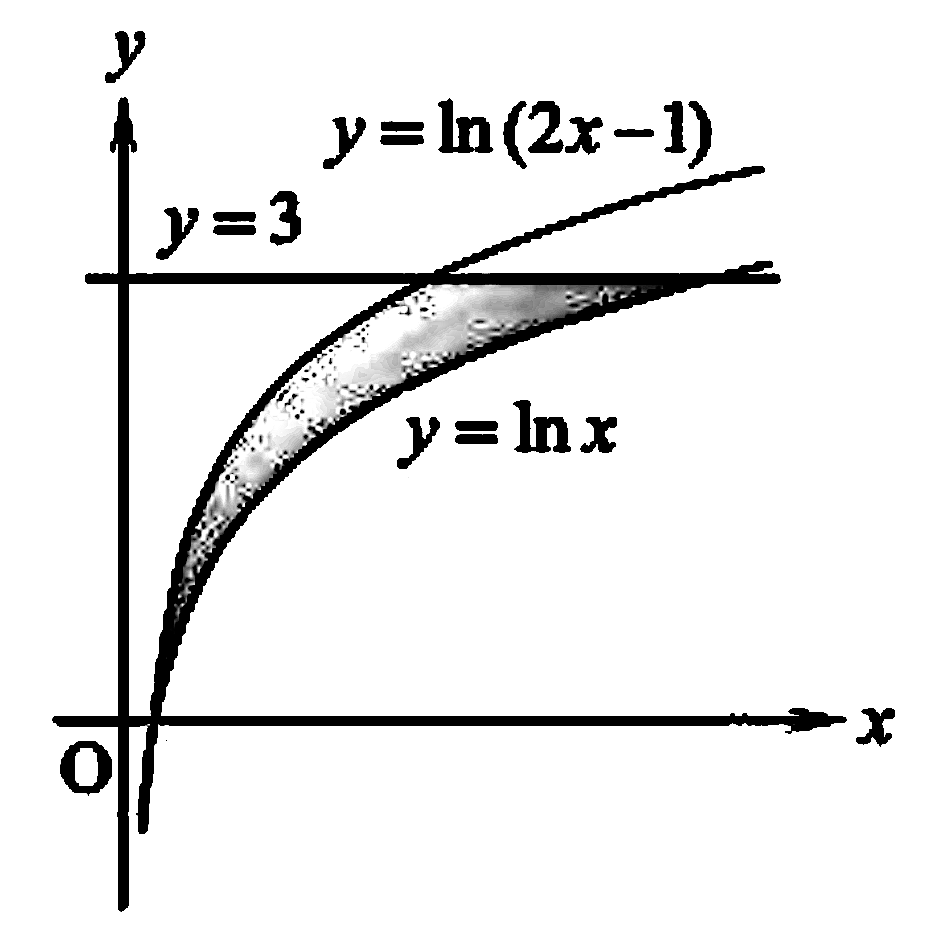
\includegraphics[scale=0.15]{assets/28-rev-28.png}
            \end{center}
            \sol{}
            \begin{flalign*}
                  y   & = \ln(2x - 1)        & \\
                  e^y & = 2x - 1             & \\
                  x   & = \dfrac{e^y + 1}{2} &
            \end{flalign*}
            \begin{flalign*}
                  y & = \ln x & \\
                  x & = e^y
            \end{flalign*}
            \begin{flalign*}
                  A & = \int_0^3 \left(e^y - \dfrac{e^y + 1}{2}\right) d y & \\
                    & = \int_0^3 \left(\dfrac{e^y - e^y - 1}{2}\right) d y & \\
                    & = \dfrac{1}{2}\int_0^3 (e^y - 1) d y                 & \\
                    & = \dfrac{1}{2}\bigg[e^y - y\bigg]_0^3                & \\
                    & = \dfrac{1}{2}(e^3 - 3 - 1)                          & \\
                    & = \dfrac{1}{2}(e^3 - 4)                              & \\
                    & = \dfrac{1}{2}e^3 - 2
            \end{flalign*}

            \newpage
      \item Find the area of the region bounded by the curves $x=y^3-y$ and $x=y-y^2$.
            \sol{}
            \begin{flalign*}
                  y^3 - y           & = y - y^2                & \\
                  y^3 + y^2 - 2y    & = 0                      & \\
                  y(y^2 + y - 2)    & = 0                      & \\
                  y(y + 2)(y - 1)   & = 0                      & \\
                  y = 0 \text{ or } & y = -2 \text{ or } y = 1
            \end{flalign*}
            \begin{flalign*}
                  A & = \int_{-2}^0 \left(y^3 - y - y + y^2\right) d y + \int_0^1 \left(y - y^2 - y^3 + y\right) d y                          & \\
                    & = \int_{-2}^0 (y^3 + y^2 - 2y) d y + \int_0^1 (-y^3 - y^2 + 2y) d y                                                     & \\
                    & = \bigg[\dfrac{1}{4}y^4 + \dfrac{1}{3}y^3 - y^2\bigg]_{-2}^0 + \bigg[-\dfrac{1}{4}y^4 - \dfrac{1}{3}y^3 + y^2\bigg]_0^1 & \\
                    & = -4 + \dfrac{8}{3} + 4 - \dfrac{1}{4} - \dfrac{1}{3} + 1                                                               & \\
                    & = \dfrac{37}{12}
            \end{flalign*}

      \item Shown in the diagram below is the shaded region bounded by the curves $y=\sin
                  x$ 及 $y=\sin 2 x$ in the interval $0 \leq x \leq \pi$. Find the area of this
            region.
            \begin{center}
                  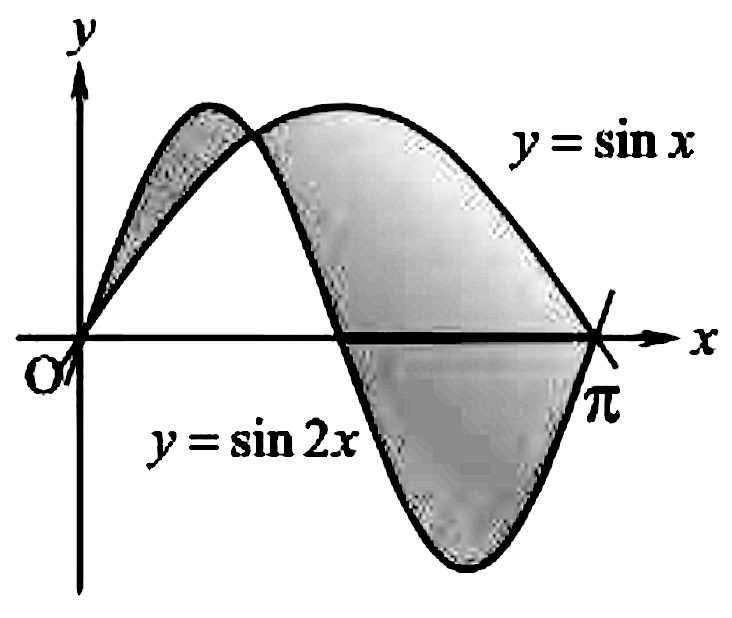
\includegraphics[scale=0.2]{assets/28-rev-30.png}
            \end{center}
            \sol{}
            \begin{flalign*}
                  \sin x                 & = 2 \sin x \cos x                      & \\
                  2\sin x\cos x - \sin x & = 0                                    & \\
                  \sin x(2\cos x - 1)    & = 0                                    & \\
                  \sin x = 0 \text{ or } & \cos x = \dfrac{1}{2}                  & \\
                  x = 0 \text{ or }      & x = \dfrac{\pi}{3} \text{ or } x = \pi
            \end{flalign*}
            \begin{flalign*}
                  A & = \int_0^{\frac{\pi}{3}} (\sin 2x - \sin x) d x + \int_{\frac{\pi}{3}}^{\pi} (\sin x - \sin 2x) d x                             & \\
                    & = \bigg[-\dfrac{1}{2}\cos 2x + \cos x\bigg]_0^{\frac{\pi}{3}} + \bigg[-\cos x + \dfrac{1}{2}\cos 2x\bigg]_{\frac{\pi}{3}}^{\pi} & \\
                    & = \dfrac{1}{4} + \dfrac{1}{2} + \dfrac{1}{2} - 1 + 1 + \dfrac{1}{2} + \dfrac{1}{2} + \dfrac{1}{4} = \dfrac{5}{2}
            \end{flalign*}

            \begin{multicols}{2}
                  \item Find the volume of the solid of revolution formed by rotating the region
                  bounded by the curve $y=\dfrac{1}{x+2}$, the line $x=2$, and two axes about the
                  $x$-axis. \sol{}
                  \begin{flalign*}
                        V & = \int_0^2 \pi\left(\dfrac{1}{x + 2}\right)^2 d x & \\
                          & = \pi\int_0^2 \dfrac{1}{(x + 2)^2} d x
                  \end{flalign*}
                  Let $u = x + 2$, then $du = dx$.

                  When $x = 0$, $u = 2$.

                  When $x = 2$, $u = 4$.
                  \begin{flalign*}
                        V & = \pi\int_2^4 \dfrac{1}{u^2} d u               & \\
                          & = \pi\bigg[-\dfrac{1}{u}\bigg]_2^4             & \\
                          & = \pi\left(-\dfrac{1}{4} + \dfrac{1}{2}\right) & \\
                          & = \dfrac{\pi}{4}
                  \end{flalign*}
                  \vfill\null
                  \item Find the volume of the solid of revolution formed by rotating the region
                  bounded by the curve $y=e^x-3$ and the two axes about the $x$-axis. \sol{}
                  \begin{flalign*}
                        e^x - 3 & = 0     & \\
                        e^x     & = 3     & \\
                        x       & = \ln 3
                  \end{flalign*}
                  \begin{flalign*}
                        V & = \int_0^{\ln 3} \pi(e^x - 3)^2 d x                                                   & \\
                          & = \pi\int_0^{\ln 3} (e^{2x} - 6e^x + 9) d x                                           & \\
                          & = \pi\int_0^{\ln 3} e^{2x} d x - \pi\int_0^{\ln 3} 6e^x d x + \pi\int_0^{\ln 3} 9 d x & \\
                  \end{flalign*}
                  Let $u = 2x$, then $du = 2dx$.

                  When $x = 0$, $u = 0$.

                  When $x = \ln 3$, $u = 2\ln 3$.
                  \begin{flalign*}
                        V & = \dfrac{\pi}{2}\int_0^{2\ln 3} e^u d u - 6\pi\int_0^{\ln 3} e^x d x + 9\pi\int_0^{\ln 3} d x            & \\
                          & = \dfrac{\pi}{2}\bigg[e^u\bigg]_0^{2\ln 3} - 6\pi\bigg[e^x\bigg]_0^{\ln 3} + 9\pi\bigg[x\bigg]_0^{\ln 3} & \\
                          & = \dfrac{\pi}{2}(9 - 1) - 6\pi(3 - 1) + 9\pi\ln 3                                                        & \\
                          & = 4\pi - 12\pi + 9\pi\ln 3                                                                               & \\
                          & = \pi(9\ln 3 - 8)
                  \end{flalign*}
                  \vfill\null
            \end{multicols}
            \vfill\null

      \item Find the volume of the solid of revolution formed by rotating the region
            bounded by the curve $x=y^2-3 y$ and the $y$-axis about the $y$-axis. \sol{}
            \begin{flalign*}
                  V & = \int_{0}^{3} \pi(y^2 - 3y)^2 d y                                & \\
                    & = \pi\int_{0}^{3} (y^4 - 6y^3 + 9y^2) d y                         & \\
                    & = \pi\bigg[\dfrac{1}{5}y^5 - \dfrac{3}{2}y^4 + 3y^3\bigg]_{0}^{3} & \\
                    & = \pi\left(\dfrac{243}{5} - \dfrac{243}{2} + 81\right)            & \\
                    & = \dfrac{81\pi}{10}
            \end{flalign*}
            \vfill\null

            \newpage
            \begin{multicols}{2}
                  \item Find the volume of the solid of revolution formed by rotating the region
                  bounded by the curve $y=x^2$ and the line $y=x+2$ about the $x$-axis.
                  \begin{flalign*}
                        x^2               & = x + 2 & \\
                        x^2 - x - 2       & = 0     & \\
                        (x - 2)(x + 1)    & = 0     & \\
                        x = 2 \text{ or } & x = -1
                  \end{flalign*}
                  \vspace{-0.5cm}
                  \begin{flalign*}
                        V & = \int_{-1}^2 \pi\left[(x + 2)^2 - x^4\right] d x                                             & \\
                          & = \pi\int_{-1}^2 (x^2 + 4x + 4 - x^4) d x                                                     & \\
                          & = \pi\bigg[-\dfrac{1}{5}x^5 + \dfrac{1}{3}x^3 + 2x^2 + 4x\bigg]_{-1}^2                        & \\
                          & = \pi\left(-\dfrac{32}{5} + \dfrac{8}{3} + 8 + 8 - \dfrac{1}{5} + \dfrac{1}{3} - 2 + 4\right) & \\
                          & = \dfrac{72\pi}{15}
                  \end{flalign*}
                  \vfill\null

                  \item Find the volume of the solid of revolution formed by rotating the region
                  bounded by the curve $y^2=x+9$ and the line $y=x+3$ about the $y$-axis. \sol{}
                  \begin{flalign*}
                        y^2 - 9           & = y - 3 & \\
                        y^2 - y - 6       & = 0     & \\
                        (y - 3)(y + 2)    & = 0     & \\
                        y = 3 \text{ or } & y = -2
                  \end{flalign*}
                  \vspace{-0.5cm}
                  \begin{flalign*}
                        V & = \int_{-2}^3 \pi\left[(y^2 - 9)^2 - (y - 3)^2\right] d y                                     & \\
                          & = \pi\int_{-2}^3 (y^4 - 18y^2 + 81 - y^2 + 6y - 9) d y                                        & \\
                          & = \pi\int_{-2}^3 (y^4 - 19y^2 + 6y + 72) d y                                                  & \\
                          & = \pi\bigg[\dfrac{1}{5}y^5 - \dfrac{19}{3}y^3 + 3y^2 + 72y\bigg]_{-2}^3                       & \\
                          & = \pi\left(\dfrac{243}{5} - 171 + 27 + 216 + \dfrac{32}{5} - \dfrac{152}{3} - 12 + 144\right) & \\
                          & = \dfrac{625\pi}{3}
                  \end{flalign*}
                  \vfill\null
            \end{multicols}
            \vspace{-0.8cm}

      \item Given that a region is bounded by the curve $y^2=8 x$ and $y=x^2$. Find the
            volume of the solid of revolution formed by rotating this region about the
            $x$-axis and the $y$-axis respectively. \sol{}
            \begin{flalign*}
                  x^4               & = 8x  & \\
                  x(x^3 - 8)        & = 0   & \\
                  x = 0 \text{ or } & x = 2
            \end{flalign*}
            \vspace{-0.8cm}
            \begin{flalign*}
                  V_x & = \pi\int_0^2 (8x - x^4) d x                & \\
                      & = \pi\bigg[4x^2 - \dfrac{1}{5}x^5\bigg]_0^2 & \\
                      & = \pi\left(16 - \dfrac{32}{5}\right)        & \\
                      & = \dfrac{48\pi}{5}
            \end{flalign*}
            When $x = 2$, $y = 4$.
            \begin{flalign*}
                  V_y & = \pi\int_0^4 \left(y - \dfrac{y^4}{64}\right) d y       & \\
                      & = \pi\bigg[\dfrac{1}{2}y^2 - \dfrac{1}{320}y^5\bigg]_0^4 & \\
                      & = \pi\left(8 - \dfrac{1024}{320}\right)                  & \\
                      & = \dfrac{24\pi}{5}
            \end{flalign*}

      \item Shown in the diagram below is the shaded region bounded by the curve $y =
                  2\cos\pi x$, the line $y = 3x$, and the $y$-axis.
            \begin{center}
                  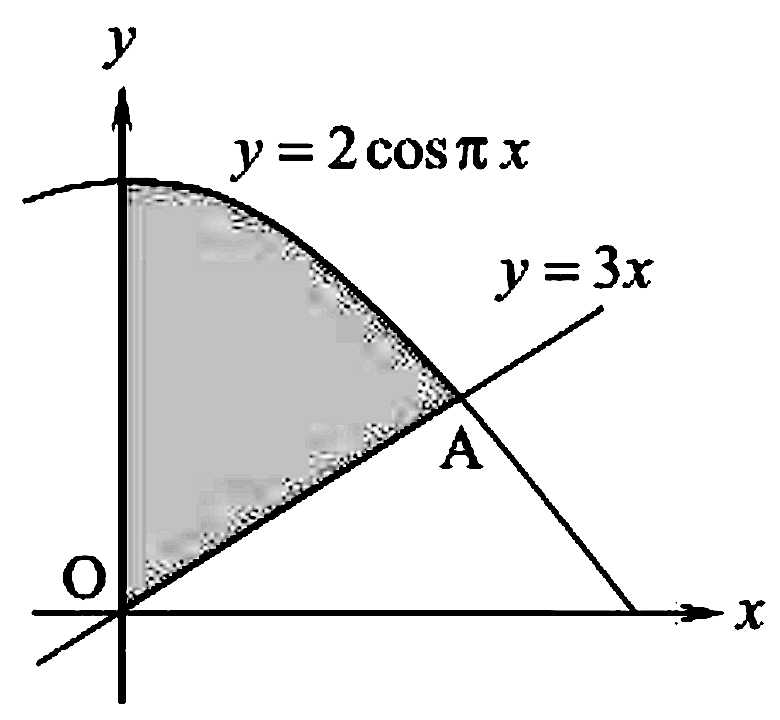
\includegraphics[scale=0.15]{assets/28-rev-37.png}
            \end{center}
            \begin{enumerate}
                  \item Prove that the $x$-coordinate of point $A$ is $\dfrac{1}{3}$. \prooff{}

                        When $x = \dfrac{1}{3}$, $y = 2\cos\left(\dfrac{\pi}{3}\right) = 1$.

                        When $x = \dfrac{1}{3}$, $y = 3\left(\dfrac{1}{3}\right) = 1$.

                        Since point $A$ is the point of intersection of the two curves, and both
                        functions give the same $y$-value when $x = \dfrac{1}{3}$, the $x$-coordinate
                        of point $A$ is $\dfrac{1}{3}$. \qed
                  \item Find the volume of the solid of revolution formed by rotating this region about
                        the $x$-axis. \sol{}
                        \begin{flalign*}
                              V & = \pi\int_0^{\frac{1}{3}} (4\cos^2\pi x - 9x^2) d x                                 & \\
                                & = \pi\int_0^{\frac{1}{3}} (2 - 9x^2) d x + 2\pi\int_0^{\frac{1}{3}} \cos 2\pi x d x
                        \end{flalign*}
                        Let $u = 2\pi x$, then $du = 2\pi dx$.

                        When $x = 0$, $u = 0$, when $x = \dfrac{1}{3}$, $u = \dfrac{2\pi}{3}$.
                        \begin{flalign*}
                              V & = \pi\int_0^{\frac{1}{3}} (2 - 9x^2) d x + \int_0^{\frac{2\pi}{3}} \cos u d u      & \\
                                & = \pi\bigg[2x - 3x^3\bigg]_0^{\frac{1}{3}} + \bigg[\sin u\bigg]_0^{\frac{2\pi}{3}} & \\
                                & = \pi\left(\dfrac{2}{3} - \dfrac{1}{9}\right) + \dfrac{\sqrt{3}}{2}                & \\
                                & = \dfrac{5\pi}{9} + \dfrac{\sqrt{3}}{2}
                        \end{flalign*}
            \end{enumerate}
      \item Given that a region is bounded by the curve $xy = 12$, the line $x = 4$, and $y
                  = 6$. Find the volume of the solid of revolution formed by rotating this region
            about the $x$-axis and the $y$-axis respectively. \sol{} \vspace{-0.8cm}
            \begin{multicols}{2}
                  \begin{flalign*}
                        V_x & = \pi\int_2^4 \left(36 - \dfrac{144}{x^2}\right) d x & \\
                            & = \pi\bigg[36x + \dfrac{144}{x}\bigg]_2^4            & \\
                            & = \pi\left(144 + 36 - 72 - 72\right)                 & \\
                            & = 36\pi
                  \end{flalign*}

                  \begin{flalign*}
                        V_y & = \pi\int_3^6 \left(16 - \dfrac{144}{y^2}\right) d y & \\
                            & = \pi\bigg[16y + \dfrac{144}{y}\bigg]_3^6            & \\
                            & = \pi\left(96 + 24 - 48 - 48\right)                  & \\
                            & = 24\pi
                  \end{flalign*}
            \end{multicols}
\end{enumerate}